\documentclass[11pt,a4paper]{article}

\usepackage[margin=2.2cm]{geometry}
\usepackage[T1]{fontenc}
\usepackage{mathptmx}
\usepackage{amsmath,amssymb}
\usepackage{booktabs}
\usepackage{graphicx}
\usepackage{microtype}
\usepackage[hidelinks]{hyperref}

\title{\textbf{GMaster methods trust}\\[0.3em]
\large Masked pseudo-\texorpdfstring{$C_\ell$}{Cl} on GPU: agreement and wall-clock vs NaMaster}
\author{GMaster development team}
\date{September 2026}

\begin{document}
\maketitle
\vspace{-1.5em}

\begin{abstract}
\noindent
We document \emph{methods trust} for GMaster, a JAX/GPU reimplementation of the NaMaster
masked pseudo-\(C_\ell\) (MASTER) estimator. The question is verifiable: on fixed maps, masks, and
binning, does GMaster reproduce NaMaster's decoupled bandpowers within numerical tolerance, and
how do wall-clocks compare? We state the estimator equations, the map\(\leftrightarrow\)alm
pipeline, and a short note on agentic development and cross-checking. Two real-map demos at
HEALPix \(N_{\mathrm{side}}=4096\)---ACT DR6 temperature and a FLAMINGO Compton-\(y\) map---show
fractional agreement at the \(10^{-5}\)--\(10^{-7}\) level and \(\sim\!9\times\) warm GPU speedups
against a 192-core NaMaster reference. This note is \emph{not} a cosmological analysis.
\end{abstract}

\section{Verifiable problem}\label{sec:problem}

Partial-sky power spectra require propagating mask mode coupling. NaMaster~\cite{namaster}
implements the MASTER decoupling of Alonso et al.~\cite{master} with a stable CPU reference
(\texttt{pymaster}). GMaster exports a NaMaster-compatible API and runs the same algebra on
accelerator arrays (JAX), targeting the full estimator chain rather than isolated transforms.

Trust is measured on \emph{fixed inputs}: identical HEALPix maps and masks, linear bandpowers
with the same \(\ell_{\max}=3N_{\mathrm{side}}-1\), Jacobi mask refinement (\(n_{\mathrm{iter}}=3\)),
and spin-0 temperature auto-spectra. We report
\begin{enumerate}
  \item fractional bandpower agreement \(C_\ell^{\mathrm{GM}}/C_\ell^{\mathrm{NM}}-1\), and
  \item wall time for field construction, coupling matrix, coupled cell, and decoupling (I/O excluded).
\end{enumerate}
No cosmological parameters, foreground models, or survey-specific science enter this document.

\section{MASTER estimator vs NaMaster}\label{sec:eqs}

For fields \(a,b\) with masks \(M_a,M_b\), pseudo-alm coefficients \(\tilde a_{\ell m}\) are
obtained by spherical harmonic analysis of \(M_a a\). The \emph{coupled} pseudo-spectrum is
\begin{equation}\label{eq:coupled}
  \tilde C_\ell^{ab} = \frac{1}{2\ell+1}\sum_m \Re\!\bigl(\tilde a_{\ell m}\,\tilde b_{\ell m}^*\bigr),
\end{equation}
with an extra factor of two for spin \(\ge 1\) as in NaMaster. Mask coupling mixes modes:
\begin{equation}\label{eq:coupling}
  \langle \tilde C_\ell^{ab}\rangle = \sum_{\ell'} M_{\ell\ell'}^{ab}\, C_{\ell'}^{ab} + \text{(noise)}.
\end{equation}
Given workspace \(M_{\ell\ell'}\), the decoupled bandpower estimate is
\begin{equation}\label{eq:decouple}
  \hat b_j = \sum_{\ell\in\mathrm{bin}\,j} W_{\ell j}\,\bigl(M^{-1}\tilde C\bigr)_\ell,
\end{equation}
with binning weights \(W_{\ell j}\) from \texttt{NmtBin.from\_lmax\_linear}. GMaster's
\texttt{NmtField}, \texttt{NmtWorkspace.compute\_coupling\_matrix}, \texttt{compute\_coupled\_cell},
and \texttt{decouple\_cell} follow NaMaster's call order and normalization; unit tests hold
matrix elements and decoupled cells to NaMaster at float64 tolerance on synthetic skies.

\section{Map\(\leftrightarrow\)alm pipeline}\label{sec:pipeline}

The timed chain mirrors NaMaster's public workflow:
\begin{enumerate}
  \item \textbf{Field.} Build \texttt{NmtField(mask, [map], n\_iter=3)}; internally analyse
        the map and (lazily) the mask with spin-0 SHTs at \(\ell_{\max}=3N_{\mathrm{side}}-1\).
  \item \textbf{Coupling.} Assemble \(M_{\ell\ell'}\) for the field pair (scalar TT uses the
        optimized recurrence; polarised cases use Gauss--Legendre quadrature).
  \item \textbf{Coupled cell.} Form \(\tilde C_\ell\) from field alms (\autoref{eq:coupled}).
  \item \textbf{Decouple.} Apply \(M^{-1}\) and bin (\autoref{eq:decouple}).
\end{enumerate}
GMaster's default scalar route at \(N_{\mathrm{side}}\ge 256\) uses a table-free latitudinal
march (float32 recurrence with float64 accumulation) and optional float32 coupling operands where
the v2 march is active; the demos below use this default production path, not a special ``exact''
override.

\section{Agentic methods sketch}\label{sec:agentic}

Implementation proceeded by (i) locking the NaMaster API surface and parity tests, (ii) replacing
kernels incrementally (coupling, SHT, ring FFT) with JAX programs checked against NaMaster on
CPU, and (iii) promoting only passes that improved wall-clock without breaking agreement gates.
Large refactors were rejected when isolated benchmarks regressed accuracy or when device memory
refused full-\(N_{\mathrm{side}}\) geometries. Real-map overlays (this note) sit above the unit
suite: they guard against footprint-specific failures that synthetic tests miss.

\section{Trust evidence: ACT and FLAMINGO}\label{sec:evidence}

\subsection{ACT DR6 temperature}

Map: ACT DR6 night PA4 f150 source-free coadd (Stokes \(I\)). Native HEALPix
\(N_{\mathrm{side}}=8192\); for this demo the map is degraded to \(N_{\mathrm{side}}=4096\) with
\texttt{healpy.ud\_grade} and cached before estimation. Mask: finite, non-zero pixels
(\(f_{\mathrm{sky}}\approx 0.48\)), identical for both codes.

\subsection{FLAMINGO Compton-\(y\)}

Map: FLAMINGO L2p8 unlensed Compton-\(y\) lightcone, full sky at \(N_{\mathrm{side}}=4096\)
(\(f_{\mathrm{sky}}=1\)).

\subsection{Results}

Both cases use \(n_{\mathrm{lb}}=50\), \(n_{\mathrm{iter}}=3\), spin 0. Warm GMaster times exclude
first-run JIT compilation; NaMaster used 192 CPU cores. NaMaster completed successfully in both
demos---no ``N/A'' fallback was required at \(N_{\mathrm{side}}=4096\) TT.

\begin{table}[ht]
  \centering
  \caption{Methods-trust summary from shipped \texttt{examples/*/README.txt} artifacts.}
  \label{tab:trust}
  \begin{tabular}{@{}lcccc@{}}
    \toprule
    Case & rms\((C_\ell^{\mathrm{GM}}/C_\ell^{\mathrm{NM}}-1)\) &
    GMaster (warm) & NaMaster & ratio \\
    \midrule
    ACT DR6 TT & \(1.4\times 10^{-5}\) & 7.6\,s & 70.4\,s & \(\sim\!9\times\) \\
    FLAMINGO \(y\) & \(2.3\times 10^{-7}\) & 8.6\,s & 69.5\,s & \(\sim\!8\times\) \\
    \bottomrule
  \end{tabular}
\end{table}

\begin{figure}[ht]
  \centering
  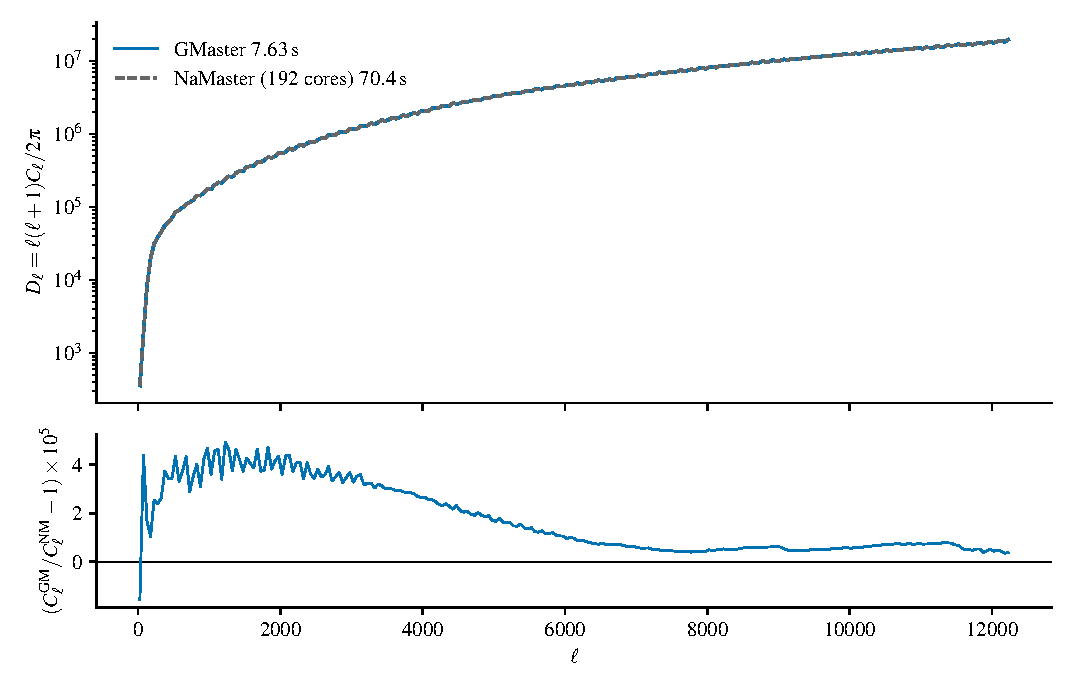
\includegraphics[width=\linewidth]{../../examples/act_dr6_tt_example/overlay.pdf}
  \caption{ACT DR6 TT: \(D_\ell\) overlay (top) and \((C_\ell^{\mathrm{GM}}/C_\ell^{\mathrm{NM}}-1)\)
  (bottom). Timings in legend from committed run logs.}
  \label{fig:act}
\end{figure}

\begin{figure}[ht]
  \centering
  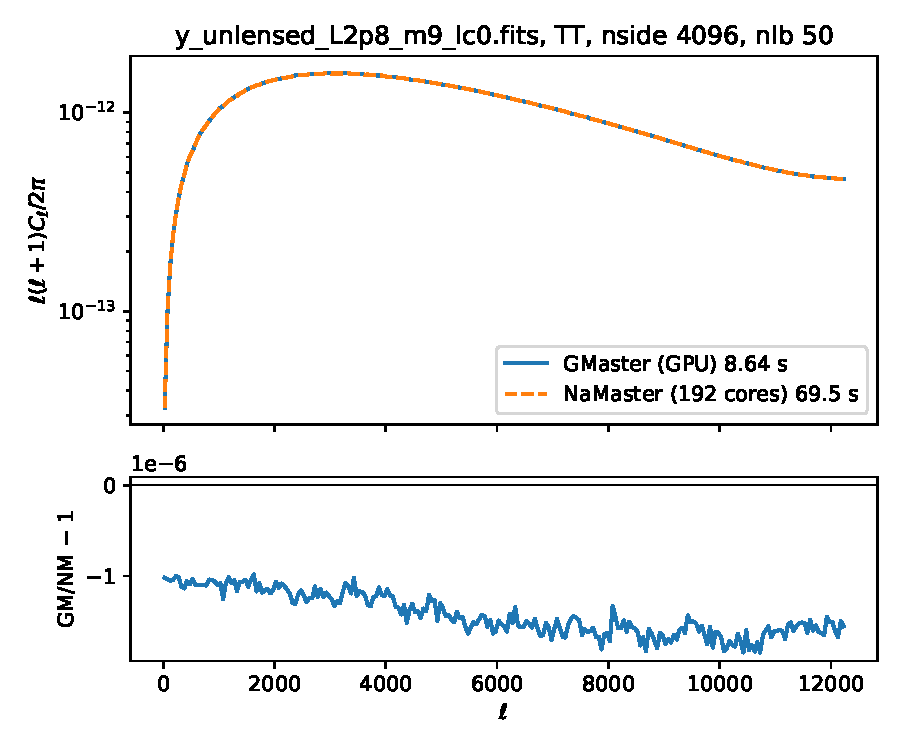
\includegraphics[width=\linewidth]{../../examples/flamingo_y_tt_example/overlay.pdf}
  \caption{FLAMINGO L2p8 Compton-\(y\) TT: same layout as \autoref{fig:act}.}
  \label{fig:flamingo}
\end{figure}

\section{Reproducing without re-running MASTER}

Committed artifacts per case: \texttt{bins.npy}, \texttt{cl\_gmaster.npy}, \texttt{cl\_namaster.npy},
\texttt{overlay.pdf}, \texttt{README.txt}. The notebook
\texttt{examples/namaster\_vs\_gmaster\_timings.ipynb} reloads these arrays and rebuilds plots and
Table~\ref{tab:trust}; it does \emph{not} invoke GMaster or NaMaster on the original FITS maps.

\appendix
\section{Minimal API snippet}\label{app:code}

\begin{verbatim}
import jax
jax.config.update("jax_enable_x64", True)
import gmaster as gm

bins = gm.NmtBin.from_lmax_linear(lmax=3*nside - 1, nlb=50)
field = gm.NmtField(mask, [temperature_map], n_iter=3)
ws = gm.NmtWorkspace()
ws.compute_coupling_matrix(field, field, bins)
cl = ws.decouple_cell(gm.compute_coupled_cell(field, field))[0]
\end{verbatim}

\begin{thebibliography}{9}
\bibitem{namaster} Alonso et al., \emph{JCAP} \textbf{08} (2019) 017; \texttt{pymaster} 3.0.
\bibitem{master} Hivon et al., \emph{ApJ} \textbf{567} (2002) 2.
\end{thebibliography}

\end{document}
